% Presentation for RSJ Annual Conference
% Author: Nishanth Koganti
% Date: 2017/01/10

\documentclass[11pt,
               hyperref={colorlinks,citecolor=pink,linkcolor=red,urlcolor=blue}
               ]{beamer}

\usetheme{default}

\usefonttheme{default}
\usecolortheme{whale}

\usepackage{bm}
\usepackage{tikz}
\usepackage{color}
\usepackage{xcolor}
\usepackage{subfig}
\usepackage{caption}
\usepackage{amssymb}
\usepackage{amsmath}
\usepackage{lmodern}
\usepackage{hyperref}
\usepackage{fancybox}
\usepackage{amsfonts}
\usepackage{listings}
\usepackage{graphicx}
\usepackage{subcaption}
\graphicspath{{./Images/}}
\usepackage[absolute,overlay]{textpos}
\usetikzlibrary{arrows,shapes,backgrounds,shapes.misc,fit}

\everymath{\displaystyle}
\setbeamerfont{footnote}{size=\tiny}

\setbeamercovered{invisible}
\setbeamercolor{footline}{fg=black}
\setbeamertemplate{blocks}[rounded]
\setbeamertemplate{navigation symbols}{}
\setbeamertemplate{footline}[frame number]
\setbeamerfont{footline}{size=\footnotesize}
\setbeamerfont{block body}{size=\footnotesize}
\setbeamertemplate{frametitle}[default][center]
\setbeamerfont{block title}{size=\footnotesize}
\setbeamercolor*{block body}{fg= white,bg= blue!60}
\setbeamercolor*{block title}{fg= white,bg= blue!70}
\setbeamerfont{block body example}{size=\footnotesize}
\setbeamerfont{block title example}{size=\footnotesize}
\setbeamercolor*{block body example}{fg=white,bg= red!60}
\setbeamercolor*{block title example}{fg=white,bg= red!70}

\newcommand{\highlight}[2][yellow]{\colorbox{#1}{$\displaystyle #2$}}
\newcommand{\tikzmark}[1]{\tikz[overlay,remember picture] \node (#1) {};}

\tikzset{square arrow/.style={to path={-- ++(0,-.25)  -| (\tikztotarget) \tikztonodes},below,pos=.25}}

\tikzstyle{line} = [draw, ultra thick, -latex']
\tikzstyle{block} = [rectangle, draw, fill=blue!20, text width=5em, text centered, rounded corners, minimum height=3em, font=\scriptsize]

\tikzstyle{block0} = [rectangle, draw, fill=blue!20, text width=5em, text centered, rounded corners, minimum height=4em]
\tikzstyle{block1} = [rectangle, draw, fill=green!20, text width=5em, text centered, rounded corners, minimum height=4em,minimum width=12em]
\tikzstyle{block2} = [rectangle, draw, text width=5em, text centered, rounded corners, minimum height=6em,minimum width=35em]
\tikzstyle{line0} = [draw, -latex']
\tikzstyle{cloud} = [draw, ellipse,fill=red!20, node distance=3cm, minimum height=2em]

\newenvironment{reference}[2]{\begin{textblock*}{\textwidth}(#1,#2) \footnotesize\it\bgroup\color{red!50!black}}{\egroup\end{textblock*}}

\title[NIPS Highlights]{Highlights of NIPS 2016}
\author[Nishanth]{Nishanth Koganti}
\institute[NAIST]{Research Student, Shibata Lab \\ \tiny{Kyushu Institute of Technology}}
\date{January 13, 2017}

\titlegraphic{
\includegraphics[height=2cm]{nipsLogo.png}\hspace*{1.5cm}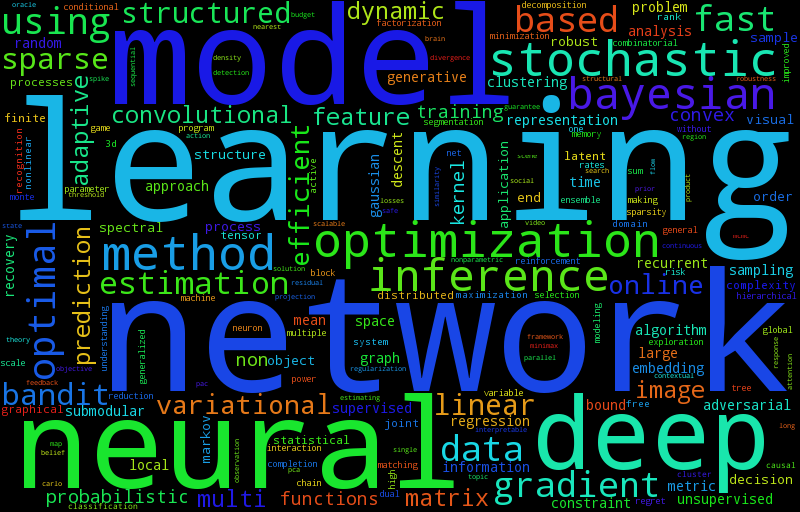
\includegraphics[height=2cm]{nipsWords.png}\hspace*{1.5cm}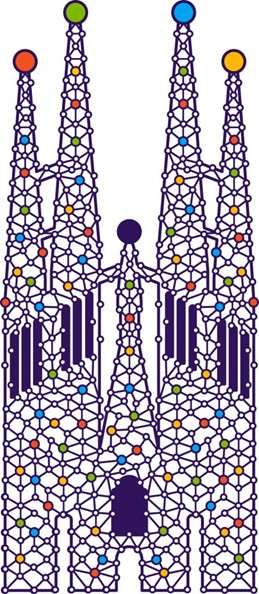
\includegraphics[height=2cm]{barcelonaLogo.jpg}}

\begin{document}

  \begin{frame}[noframenumbering]
    \titlepage
  \end{frame}

  \section{NIPS Conference}

  \subsection{History}

  \begin{frame}
    \frametitle{Neural Information Processing Systems}

    \begin{itemize}
      \item Largest International Conference on Machine Learning.
      \item Held since 1987 and initially focused on Neural Network research.
    \end{itemize}

    \begin{figure}
      \centering
      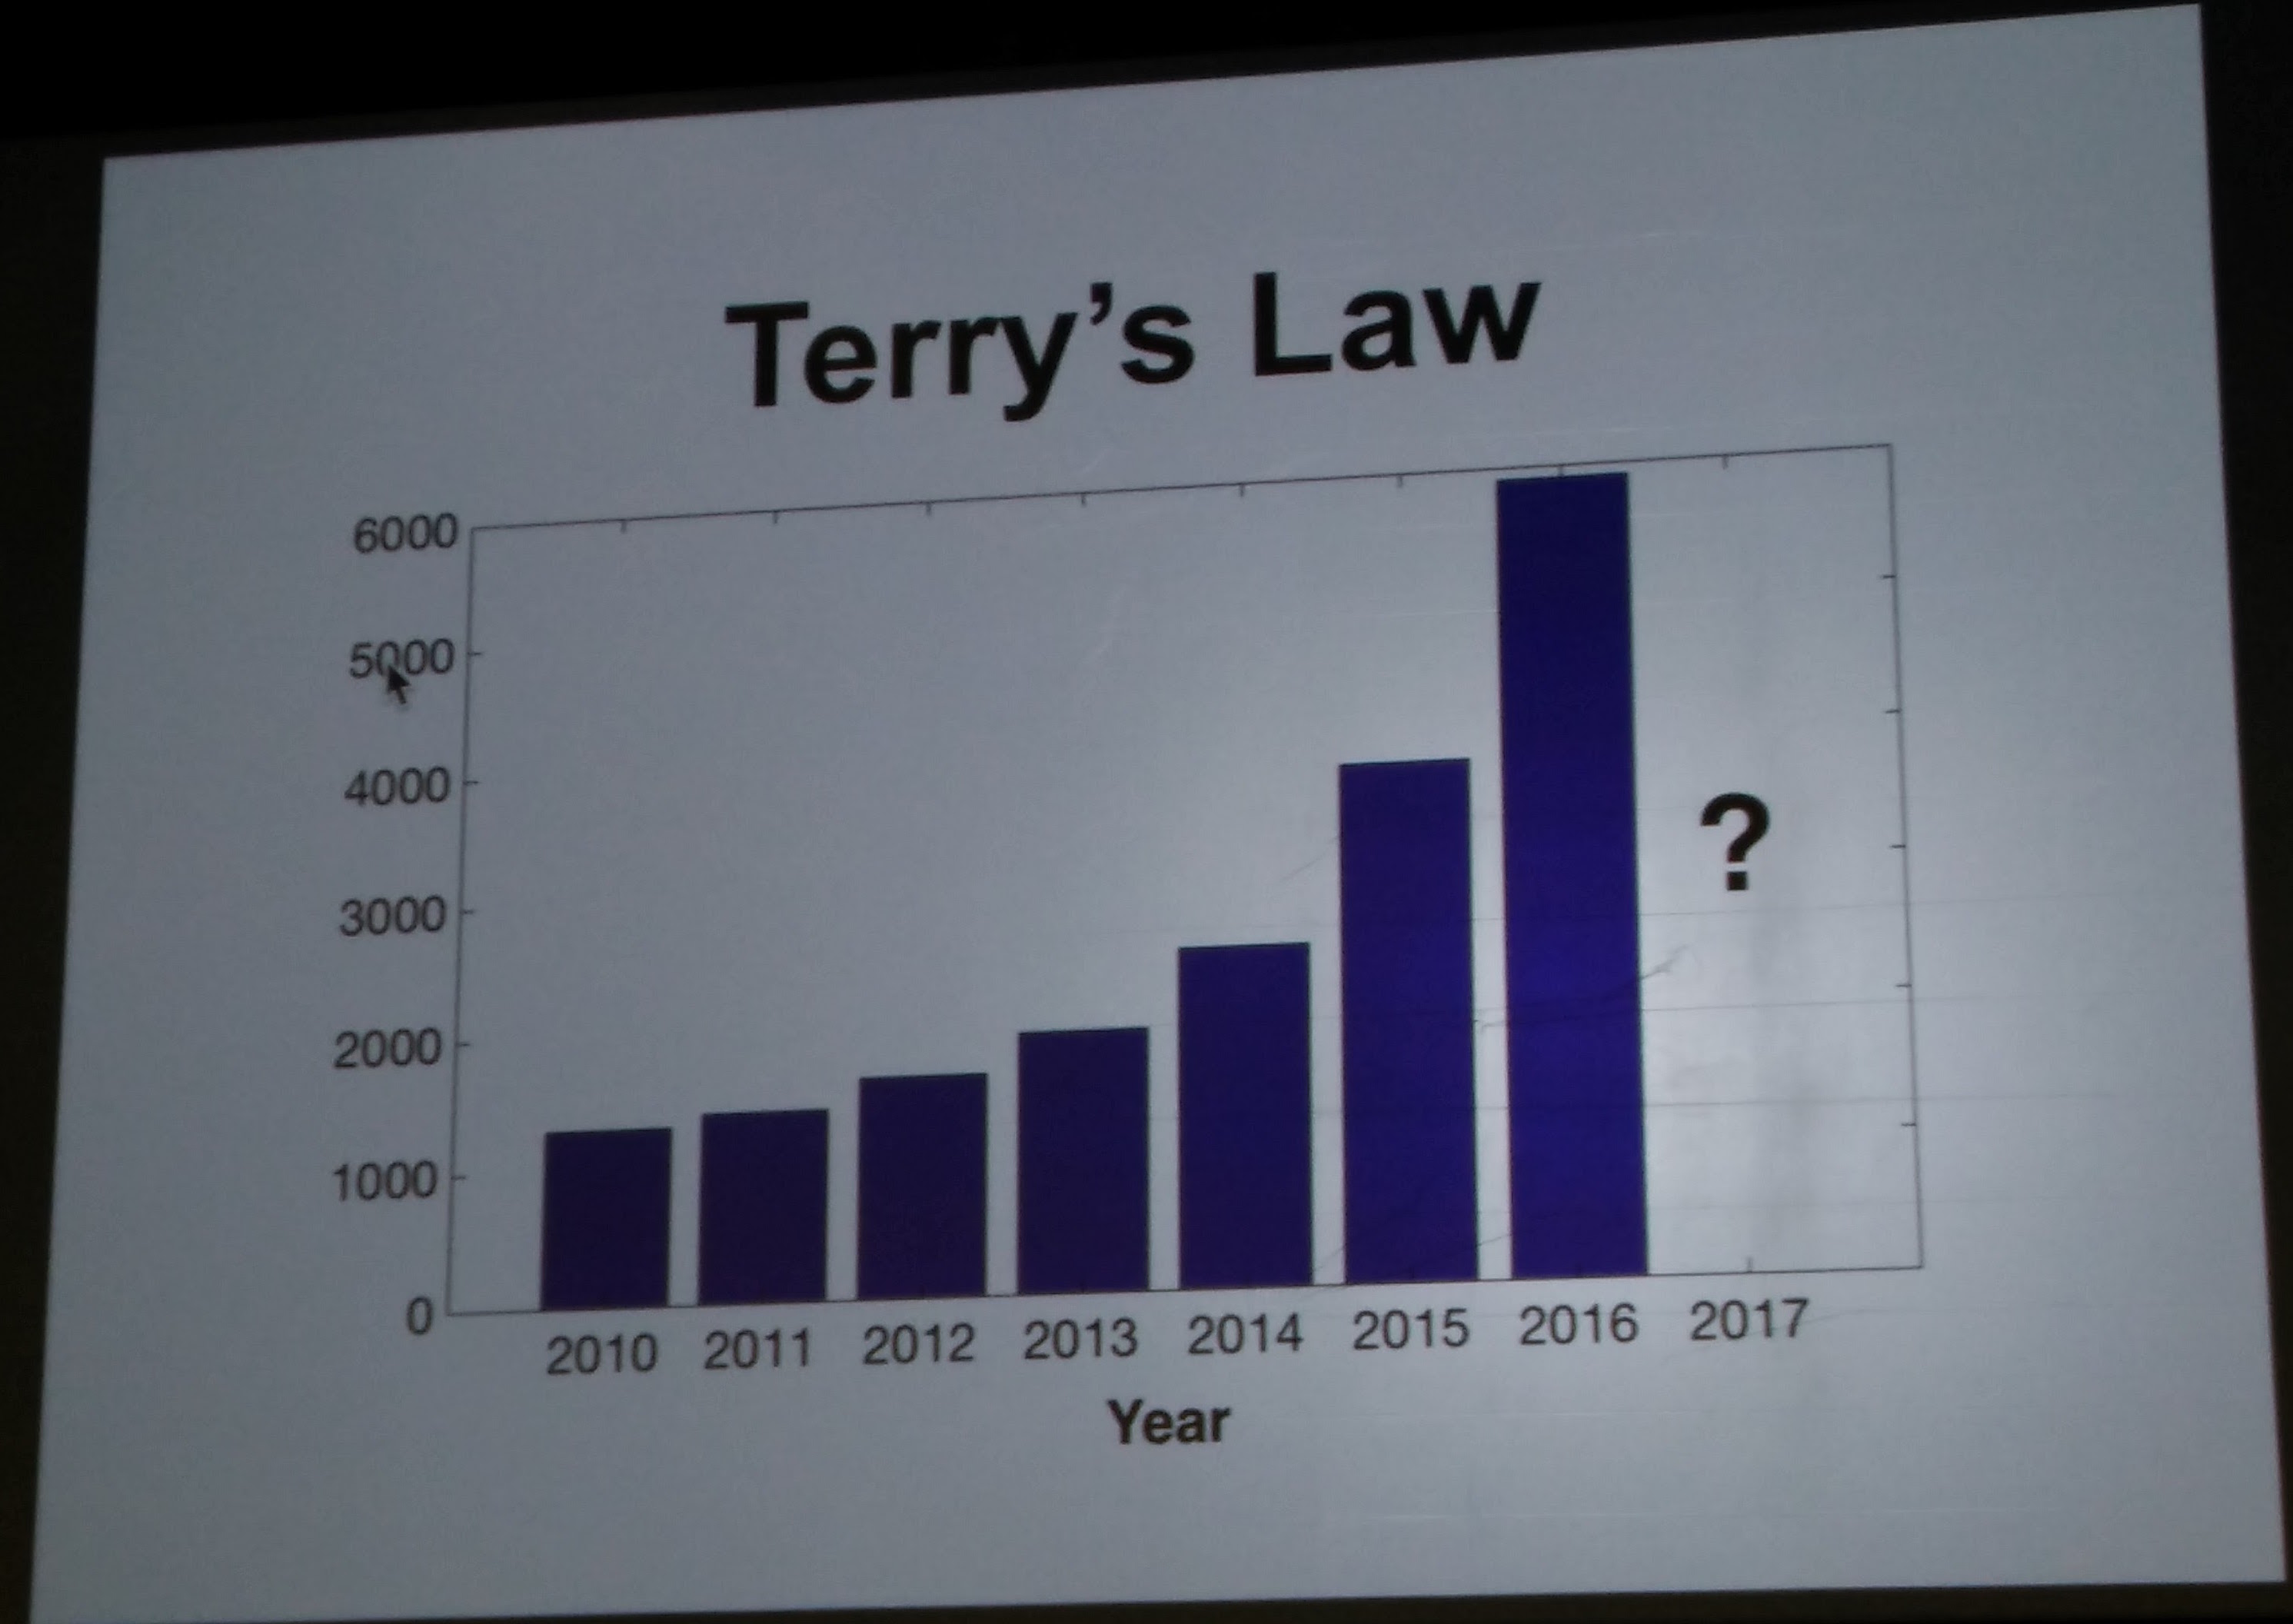
\includegraphics[width=0.65\textwidth]{terryLaw.jpg}
      \caption*{Terry's Law on NIPS Participants \footnotemark[1]}
    \end{figure}

    \footnotetext[1]{Proposed by \href{http://www.salk.edu/scientist/terrence-sejnowski/}{Terrence Sejnowski}, NIPS 2016 Chair}
  \end{frame}

  \subsection{Statistics}

  \begin{frame}
    \frametitle{NIPS 2016: Topics Convered}

    \begin{itemize}
      \item 568 Papers (46 oral) accepted among 2400 papers with 6 reviewers per submission.
      \item Most popular topics were Deep Learning (1 in 4) with application to Computer Vision (1 in 10).
    \end{itemize}

    \begin{figure}
      \centering
      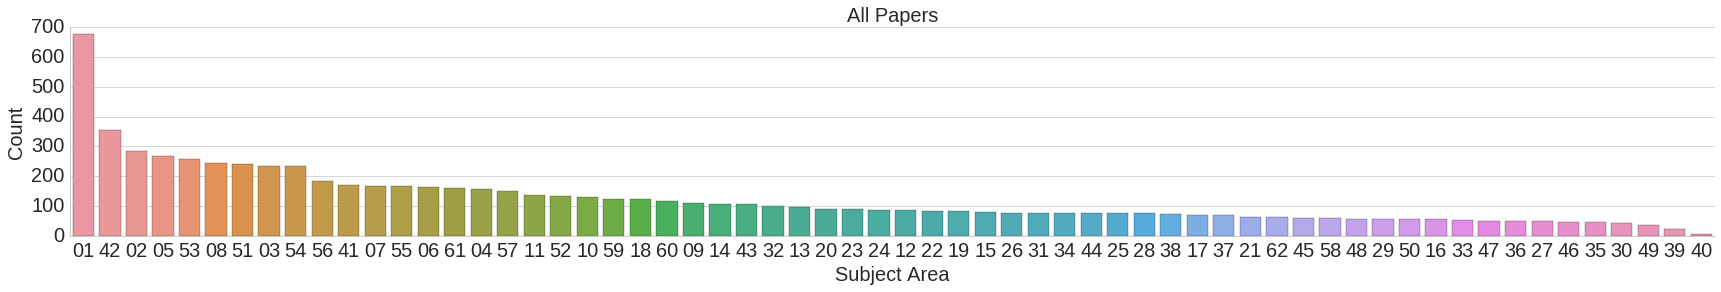
\includegraphics[width=\textwidth]{nipsTopics1.png}
    \end{figure}

    \begin{figure}
      \centering
      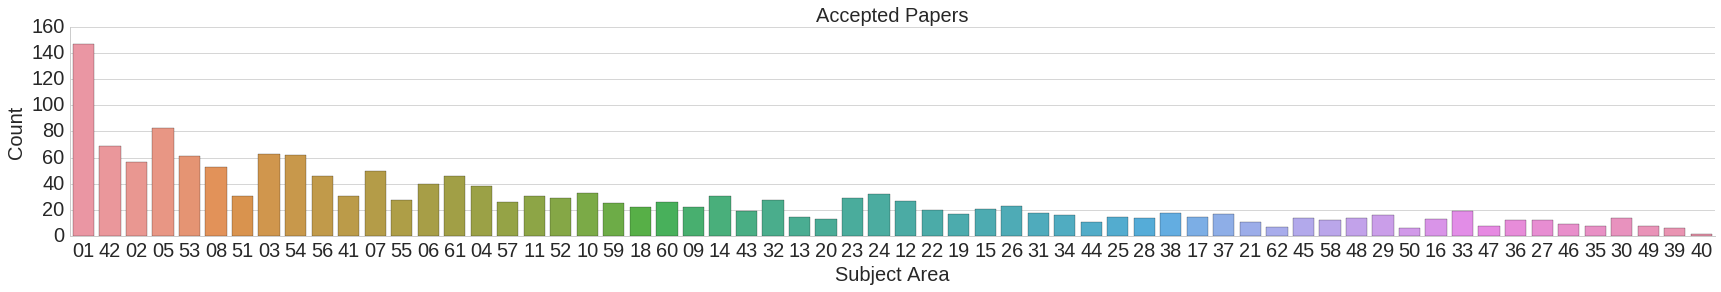
\includegraphics[width=\textwidth]{nipsTopics2.png}
      \caption*{Long-tailed Distribution of Topics \footnotemark[1]}
    \end{figure}

    \footnotetext[1]{\href{http://www.tml.cs.uni-tuebingen.de/team/luxburg/misc/nips2016/index.php}{NIPS 2016 Review Process}}
  \end{frame}

  \subsection{Impressions}

  \begin{frame}
    \frametitle{NIPS 2016: Impressions}

    \begin{itemize}
      \item
    \end{itemize}

    %\footnotetext[1]{}
  \end{frame}

  \section{Deep Learning}

  \subsection{Generative Adversarial Networks}

  \begin{frame}
    \frametitle{Generative Adversarial Networks: Overview}

    %\footnotetext[1]{}
  \end{frame}

  \begin{frame}
    \frametitle{GAN: Tutorials}

    %\footnotetext[1]{}
  \end{frame}

  \begin{frame}
    \frametitle{GAN: Applications}

    %\footnotetext[1]{}
  \end{frame}

  \subsection{Bayesian Deep Learning}

  \begin{frame}
    \frametitle{Bayesian Deep Learning}

    %\footnotetext[1]{}
  \end{frame}

  \begin{frame}
    \frametitle{Deep Learning and Graphical Models}

    %\footnotetext[1]{}
  \end{frame}

  \begin{frame}
    \frametitle{Dropout as a Bayesian Approximation}

    %\footnotetext[1]{}
  \end{frame}

  \subsection{Deep Reinforcement Learning}

  \begin{frame}
    \frametitle{Deep Reinforcement Learning: Tutorials}

    %\footnotetext[1]{}
  \end{frame}

  \begin{frame}
    \frametitle{Deep Reinforcement Learning: Workshop}

    %\footnotetext[1]{}
  \end{frame}

  \begin{frame}
    \frametitle{Value Iteration Networks}

    %\footnotetext[1]{}
  \end{frame}

  \subsection{Recurrent Neural Networks}

  \begin{frame}
    \frametitle{Recurrent Neural Networks: Overview}

    %\footnotetext[1]{}
  \end{frame}

  \begin{frame}
    \frametitle{RNN: Symposia}

    %\footnotetext[1]{}
  \end{frame}

  \begin{frame}
    \frametitle{RNN: Applications}

    %\footnotetext[1]{}
  \end{frame}

  \subsection{Meta-learning}

  \begin{frame}
    \frametitle{Learning to learn: Meta-learning}

    %\footnotetext[1]{}
  \end{frame}

  \begin{frame}
    \frametitle{One-shot Learning}

    %\footnotetext[1]{}
  \end{frame}

  \subsection{Neural Turing Computers}

  \begin{frame}
    \frametitle{Neural Turing Machines: Overview}

    %\footnotetext[1]{}
  \end{frame}

  \begin{frame}
    \frametitle{NTM: Applications}

    %\footnotetext[1]{}
  \end{frame}

  \section{General Topics}

  \begin{frame}
    \frametitle{Nuts and Bolts of ML}

    %\footnotetext[1]{}
  \end{frame}

  \begin{frame}
    \frametitle{General AI: Unsupervised Learning}

    %\footnotetext[1]{}
  \end{frame}

  \begin{frame}
    \frametitle{Boston Robotics Demo}

    %\footnotetext[1]{}
  \end{frame}

  \begin{frame}
    \frametitle{Efficient seeding for K-Means}

    %\footnotetext[1]{}
  \end{frame}

  \begin{frame}
    \frametitle{RocketAI: The AI Bubble}

    %\footnotetext[1]{}
  \end{frame}

  \section{Visitng Barcelona}

  \begin{frame}
    \frametitle{Sightseeing in Barcelona}

  \end{frame}

  \begin{frame}[noframenumbering]

    \begin{center}
      \Huge{Thank you!}\\~\\
      \huge{Questions or Comments?}
    \end{center}
  \end{frame}

\end{document}
